%!TEX root = ../thesis.tex
%*******************************************************************************
%****************************** Fourth Chapter *********************************
%*******************************************************************************

\chapter{Benchmark}
\label{chap:benchmark}
\ifpdf
    \graphicspath{{Chapter4/Figs/Raster/}{Chapter4/Figs/PDF/}{Chapter4/Figs/}}
\else
    \graphicspath{{Chapter4/Figs/Vector/}{Chapter4/Figs/}}
\fi

\topic{Il faut un benchmark solide pour comparer les méthodes}

Plan :
\begin{itemize}
	\item Higgs data : \autoref{sec:higgs_data} describe the dataset/problem that motivated this work
	\item Toy data : \autoref{sec:toy_datasets} describe the toy dataset to explain behaviour of the methods
	\item Bayesian inference : \autoref{sec:bayesian_inference_on_toys} describe a quick way to get best inference with likelihood
	\item Constraint / Calibration : \autoref{sec:constraining_nuisance_parameters} the issue and freedom taken to choose the constraint on $\alpha$
	\item Training : \autoref{sec:training_details} how the methods are trained
	\item Evaluation : \autoref{sec:higgs_data} methods are evaluated using MSE, Vstat, Vsyst, Hesse vs Minos.
\end{itemize}






\section{Higgs data} % (fold)
\label{sec:higgs_data}



\victor{NOTE : Higgs to tau tau in ATALS start page : \url{https://atlas.lal.in2p3.fr/physics/past-activities/htautau/}}
\victor{NOTE : did we found no higgs in the H to tautau ? \url{https://journals.aps.org/prl/pdf/10.1103/PhysRevLett.125.051801}}


\subsection{Simulation} % (fold)
\label{sub:simulation}

Precise simulation is not only used for training machine learning models.
Simulation is critical for the design of the apparatus itself or planning an upgrade of the apparatus.
Simulation allows to predict how the data should be according to a given version of the standard model.
Theorists updates on the standard model can be validated or rejected efficiently by comparing their predictions through simulation to the data.

Of course simulation of an experiment at the LHC requires tremedous work.
For example the ATLAS simulation \cite{Aad_2010} can be broken down into 3 major steps.
First the event simulation that takes care of the collision, the particles creation, the particle interactions between themselves and their decay to other particles.
Second the interaction between the particles and matter (the apparatus) which is done using Geant4 \cite{AGOSTINELLI2003250}, \cite{1610988}, \cite{ALLISON2016186}.
This is the part I find the most impressive.
Sensors, magnetic field generated by the electronics, cables, even the air or the cooling liquids are taken into account.
Finally digitization deals with what numbers will come out of the previous interaction to be finally stored for later analysis.
Although very accurate simulations of all parts and phenomena is technically possible the computation power often limits its usage to more approximative ones. 
This leads to creating a custom tradeoff for each analysis to focus computation on the most relevant parts.

Interaction between particles and the sensors are again fundamentally stochastic.
A very large number of sensors is required to reach a high enough resolution to make accurate measurements.
As a consequence each sensor interaction with a particle creates a latent variable in the modeling of a single event.
Therefore 100 000 detector pieces lead to 100 000 latent variables making the marginal likelihood intractable (see \autoref{sub:inverse_problem}).

Simulation is expensive and possible processes include very rare events like Higgs boson creation.
Without \emph{importance sampling}\needcite it would be impossible to simulate enough events to get a representative sample of those rare processes.
Simulation runs independently for every processes.
Then the data are gathered with importance weights reprensenting their relative probability of occurrence.








\subsection{HiggsML challenge} % (fold)
\label{sub:higgsml_challenge}


The data were initially produced for the HiggsML challenge \cite{Adam-Bourdarios2014}.
It was a the most successfull challenge of its time with (some number of teams and submissions).
The data is now publicly available \needcite.
\victor{TODO : citer les autres articles qui ont utilisés HiggsML}

The HiggsML dataset is composed of 818238 events described by 17 primary features and 13 features derived from the primaries.
Near the end of the challenge X more constructed features known as "cooked features" became popular \needcite.
The cooked features help getting good classification perfomances\needcite in some context (what context ?).
The label designing if the event is a signal ($H\to \tau \tau$) or a backgroud (any other process) is of course available in the dataset as well.

Sample weights used for the kaggle challenge is not the same ... why again ?







\subsection{Fast re-simulator} % (fold)
\label{sub:fast_re_simulator}


In order to ease experiments, the first part of this work is to build a fast re-simulator of the events.
Indeed one event require on min of CPU time to be generated.
Regenerating the entire dataset for all the set of parameters values we might want to try would be too expensive.
However the parameters considered in this work only affect some of the final parts of the simulation and can be computed a posteriori.

A small library was published\needcite and a more recent version is available here\needcite.
This rest of this section will briefly explain how the event are re-generated for a different set of parameters.

The parameter of interest $\mu$ is the deviation of the expected number of signal from the predictions of the standard model.
Recomputing the data only requires to multiply the sample weights of the signal events with $\mu$.
This is already enough to build a complete workflow of the inference without nuisance parameter.

5 nuisance parameters are considered : tau energy scale, lepton energy scale, jet energy scale, soft term, nasty backgrounds.



\subsubsection{Energy scales} % (fold)
\label{ssub:energy_scales}

The tau energy scale is comming from apparatus imperfections leading to a slightly wrong scale of the measured energy of tau particle.
The lepton and jet energy scale are exactly analogus but with lepton particle and jets.
The 3 energy scales are independant from each other leading to 3 nuisance parameters $\alpha_{tes}, \alpha_{les}, \alpha_{jes}$. 
This nuisance parameter is basically a proportional factor on one or several primary features (eg. PRI\_tau\_pt) stained with non negligeable uncertainty.
Recomputing the events for a different value of the energy scale requires not only to multiply the primary features with the updated value but also all the features derived from this primaries.



\subsubsection{Soft term} % (fold)
\label{ssub:soft_term}

The missing energy transverse (met) is perturbated by a random vector sampled from a normal distribution which standard deviation is our nuisance parameter $\alpha_{st}$.
This is a more difficult systematic effect to infer from the data.
Just like the parameter of interest it isby definition impossible to infer the soft term from one example.




\subsubsection{Nasty background} % (fold)
\label{ssub:nasty_background}

The background distribution is a mixture of several processes.
The mixture coefficient of one of these processes is not known with enough precision.
\victor{c'est celui avec un detailLabel = W}
This nuisance parameter $\alpha_{nb}$ only requires to recompute the weights.
Since the parameter of interest is also linked with the sample weights, ie the amount of events, this nuisance parameter directly leads to an increase of the variance of our estimator $\hmu$.
Indeed a larger number of events in a bin can now be explained by an increase of $\mu$ or an increase of $\alpha_{nb}$.




\subsubsection{Mass MMC} % (fold)
\label{ssub:mass_mmc}

Unfortunately the MMC mass (what the hell is it ?) cannot be easilly recomputed from primaries.
Computing the MMC mass involves an expensive optimization step \victor{More details ?}.
Although DER\_Mass\_MMC is the a relevant feature (\textbf{see missing figure}) for classification it is removed from the dataset.

\victor{TODO : figure top 5 or top 10 feature importances}




\subsubsection{The cut at 22GeV} % (fold)
\label{ssub:the_cut}






\subsubsection{Bootstraping} % (fold)
\label{ssub:boostraping}


Re-generating the data is not the same as re-running the simulation.
\victor{Results on boostrapping that says when it is OK to do it ?}

Training the direct regression method requires way more data than training a classifier since a sample for a regressor is composed of thousands of events.
With boostrapping and considering the re-generation as data augmentation the finite HiggsML dataset can be turned into an almost infinite generator of events.












\section{Toy datasets} % (fold)
\label{sec:toy_datasets}


Toy datasets allow a full control of the generative process and the properties of the data.
It is a necessary step to produce a test bed of the program code.
But also to evaluate the influence of many parameter (eg. number of dimension, number of sample, signal/background separability, etc) on the performances to help explain the performances on real data.






\subsection{Toy 1D} % (fold)
\label{sub:toy_1d}


\isabelle{C'est la base ! Le reste est envoyé sur du 1D de toute façon.}

The first toy is a very simple case of estimation of a mixture coefficient in the presence of one systematic effect.
The likelihood is known and tracktable making maximum likelihood and bayesian inference possible.
Comparing the inference methods to the best possible inference is a first step to validate them.


The toy generative process is a mixture of 2 distributions with one observable $x \in \RR$.
The background distribution is a gamma distribution versus a gaussian distribution for the signal process.
\autoref{fig:minitoy_distrib} presents the data distribution.
To make the problem non trivial and correspond more to reality the signal distribution is overlapping with the background distribution.

The parameter of interest is the mixing coefficient $\mu$ of the 2 distributions.
The nuisance parameter $\alpha$ is a rescaling of the observable $x$.

Without nuisance parameter $\alpha$ the likelihood is :
$$
    p(x | \mu) = \mu \mathcal N(x|a, d) + (1-\mu) \Gamma(x|k, l)
$$

with $N(x|a, d)$ a gaussian with mean $a$ and standard deviation $d$ and $\Gamma(x|k, l)$ a gamma distribution with $k$ ... and $l$ the localization  ... ????
The chosen values are : $a = 5, d=0.5, k=2, l=0$.


Including nuisance parameter $\alpha$ the likelihood becomes :
$$
    p(x | \mu, \alpha) = \mu \mathcal N(x|\alpha a, \alpha d) + (1-\mu) \Gamma(x|\alpha k, l)
$$

\begin{figure}[htb]
    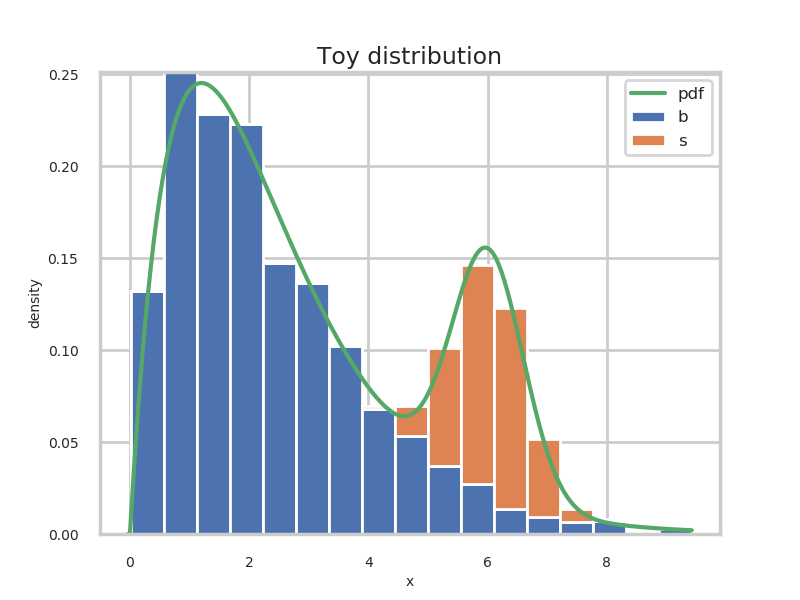
\includegraphics[width=\linewidth]{minitoy/distrib.png}
    \caption{Data distribution of the 1D toy for a 10,000 instances sampling}
    \label{fig:minitoy_distrib}
\end{figure}






\subsection{Toy 3D} % (fold)
\label{sub:toy_3d}

To get closer to reality the toy example introduced in \cite{DECASTRO2019170inferno} is also included.
It is a mixture of 2 processes : $f_b$ for the backgrounds and $f_s$ for the signals.

\begin{equation}
	f_b (x|r, \lambda) = \mathcal N \left ( (x_0, x_1) | (2+r, 0) 
	\begin{bmatrix} 5 & 0 \\ 0 & 9 \end{bmatrix} \right ) Exp((x_2| \lambda)
\end{equation}
\begin{equation}
	f_s (x|r, \lambda) = \mathcal N \left ( (x_0, x_1) | (1, 1) 
	\begin{bmatrix} 1 & 0 \\ 0 & 1 \end{bmatrix} \right ) Exp((x_2| 2)
\end{equation}

Leading to the likelihood :
\begin{equation}
	p(x | r, \lambda, \mu ) = (1-\mu) f_b(x|r, \lambda) + \mu f_s(x|r, \lambda)
\end{equation}

This toy is multi dimensional, more complex and includes 2 nuisance parameters.
The nuisance parameters affects only the background distribution.
Once again the background and signal distribution are overlapping.
\autoref{fig:s3d2_pairgrid} shows the distributions of a sampled dataset.

\begin{figure}[htb]
    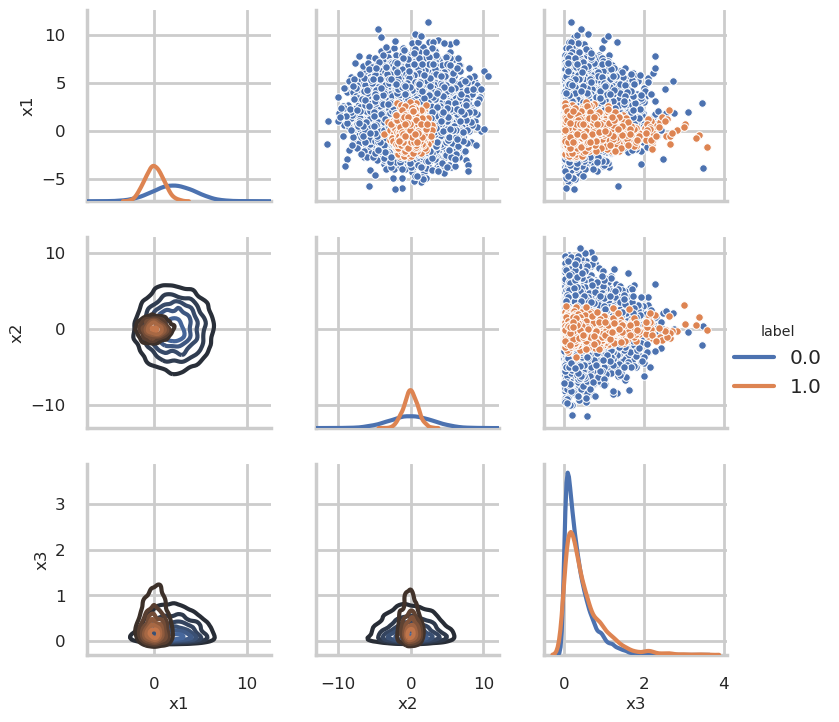
\includegraphics[width=\linewidth]{s3d2/pairgrid}
    \caption{Data distribution of the 3D toy}
    \label{fig:s3d2_pairgrid}
\end{figure}












\section{Bayesian inference on toys} % (fold)
\label{sec:bayesian_inference_on_toys}


The toy problems (see \autoref{sub:toy_1d} and \autoref{sub:toy_3d} ) do not suffer from intractable likelihood making it possible to compute the posterior probability using standard bayesian inference.
The computed posterior is the best possible inference and will be compared with the other methods that assumes the samplewise likelihood is intractable.

\subsection{Computing the posterior} % (fold)
\label{sub:computing_the_posterior}

The marginal posterior probability density function of the parameter of interest $p(\mu|D)$ can be computed from the likelihood and a prior.
The prior is chosen as uniform over the domain of possible values of the parameters $\mu$ and $\alpha$.
A dataset $D$ of independant and identically distributed samples is assumed to be available.

From Bayes theorem : 
\begin{equation}
    p(\mu, \alpha | D) = \frac{p(D|\mu, \alpha) p(\mu, \alpha)}{p(D)} = \frac{p(D|\mu, \alpha) p(\mu, \alpha)}{\int_{\alpha, \mu} p(D|\alpha, \mu) p(\mu, \alpha) d\alpha d\mu}
\end{equation}
and
\begin{equation}
	p(\mu|D) = \int_{\alpha} p(\mu, \alpha | D) p(\alpha|D) d\alpha
\end{equation}

Computing the integrals by hand can be tedious.
The inference can be approximated with a fine discretization of the continuous space of parameter.
It starts with a grid $\{\mu_i, \alpha_j\}_{i,j}$, fine enough, covering the space of possible values of the parameters.

Then we can compute the likelihood
\begin{equation}
	p(D|\mu_i, \alpha_j) = \prod_{x_k\in D} p(x_k|\mu_i, \alpha_j)
\end{equation}
Dealing with products of probabilities leads to numerical instability.
The number of samples can easily be big enough to obtain numbers too small to be precisely stored in a 64 bits float.
The usual trick is to work with log probabilities which gives the following tensor 
\begin{equation}
	L_{ij} = \log (p(D|\mu_i, \alpha_j)) = \sum_{x_k\in D} \log (p(x_k|\mu_i, \alpha_j))
\end{equation}
Combining it with a prior tensor $K_{ij} = \log(p(\mu_i, \alpha_j))$ the tensor $ R_{ij} = \log(p(D|\mu_i, \alpha_j)) + \log(p(\mu_i, \alpha_j) )$ gives access to the posterior $p(\mu_i, \alpha_j | D)$ through renormalization with $p(D)$.
Recall that :
\begin{equation}
    p(D) = \int_{\alpha, \mu} p(D|\alpha, \mu) p(\mu, \alpha) d\alpha d\mu
\end{equation}
Which gives after discretization
\begin{equation}
    p(D) = \sum_{\alpha_j, \mu_i} p(D|\alpha_j, \mu_i) p(\mu_i, \alpha_j)
\end{equation}
\begin{equation}
	T_{ij} = p(\mu_i, \alpha_j | x) = softmax(R_{ij}) = \frac{ e^{ R_{ij} }  }{ \sum_{ij} e^{ R_{ij} } }
\end{equation}

The marginal probabilities are computed from $T_{ij}$ :
\begin{equation}
	p(\mu_i | D) = \sum_j T_{ij} = M_i
\end{equation}
\begin{equation}
  p(\alpha_j | D) = \sum_i T_{ij} = A_j
\end{equation}
The method presented here is quite simple but leads to very accurate estimation on the toy problems.





\subsection{Extract quantities from discretized marginal posterior} % (fold)
\label{sub:extract_quantities_from_discretized_marginal_posterior}

A plot of $p(\mu | D)$ is not the best way of comparing the bayesian inference to the other methods.

If the distribution $p(\mu | D)$ is well behaving the expectation of $\mu$ will be close to the maximum.
\begin{equation}
	\hat\mu = \EE[\mu|D] = \sum_i \mu_i M_i
\end{equation}
The confidence interval is then the variance
\begin{equation}
	\VV(\mu|D) = \sum_i \mu_i^2 M_i - (\sum_i \mu_i M_i)^2
\end{equation}

This variance can be splitted into two contribution : the statistical variance $\EE_{\alpha \sim p(\alpha|x)}[ \VV(\mu|x, \alpha) ]$ and the systematic variance $\EE_{\alpha \sim p(\alpha|D)} \left ((\EE [\mu|D, \alpha]  - \EE[\mu|D])^2\right )$

\begin{align}
	\EE_{\alpha \sim p(\alpha|D)}[ \VV(\mu|D, \alpha) ] 
			&= \sum_j \VV(\mu|D, \alpha_j) p(\alpha_j | x) \\
			&= \sum_j \VV_i(\mu_i, \frac{T_{ij}}{A_j}) A_j
\end{align}
\begin{align}
	\EE_{\alpha \sim p(\alpha|D)} \left ((\EE [\mu|D, \alpha]  - \EE[\mu|D])^2\right ) 
			&= \VV(\mu|D) - \EE_{\alpha \sim p(\alpha|D)}[ \VV(\mu|D, \alpha) ] \\
			&= \VV(\mu_i, M_i) - \sum_j \VV_i(\mu_i, T_{ij}) A_j
\end{align}

\subsubsection{Note 1}

The neural network regressor is learning to compute either $p(\mu_i |D, \alpha_j) = \frac{p(\mu_i, \alpha_j | D)}{p(\alpha_j | D)} = \frac{T_{ij}}{A_j} = N_{ij}$ or $p(p(\mu_i |D) = = \sum_j T_{ij} = M_i$
Meaning that it is possible to compare the MDN regressor output to the true distribution.


\subsubsection{Note 2}

If there is multiple nuisance parameters $\alpha$, $\beta$, etc the tensor are simply n-dimensional : $L_{ijk...}$, $T_{ijk...}$, $K_{ijk...}$, etc.
And all sums over $j$ become sums over $j,k, ...$ which is easy to handle with broadcasting in modern numeric libraries.











\section{Constraining nuisance parameters} % (fold)
\label{sec:constraining_nuisance_parameters}




\victor{TODO : Explain how the 2 constraints are chosen, where it happen in computation of studied quantities}
\victor{TODO : Show that the new calibration is a good fit.}

At some point a constraint on the nuisance parameters $\alpha$ is requiered to avoid mutliple maxima of the likelihood.
The constraint act as a guide to find the maximum of the likelihood.
Knowing the range of possible $\alpha$ is also required to train the robust methods.

Here is desccribed how the two contraints methods considered is computed.


\subsection{Prior knowledge} % (fold)
\label{sub:prior_knowledge}


As explained in \autoref{sub:calibration_experiment} a side experiment gives access to some measurement $D_{calib}$ which depends only on $\alpha$.
This experiment leads to a estimation of $\alpha$ in the form of a posterior distribution $p(\alpha | D_{calib}$.
Most of the time these distribution are gaussian \needcite.

Unfortunatelly these calibration measurement are not included in our simulators neither on the toys nor on the higgs data.
The constraints then takes the form of a prior distribution.

Although the toy problem shares properties with some real physic experiment they do not represent any real process.
A prior distribution is pulled out of the hat.
For the higgs dataset the values are chosen to be quite close to reality \needcite.
\victor{Maybe \url{https://cds.cern.ch/record/1493615/files/HIG-12-043-pas.pdf} is a good start.}




\url{http://cds.cern.ch/record/1306523/files/CERN-2011-006.pdf?version=1} Page 115 is a good read.






























\section{Training details} % (fold)
\label{sec:training_details}

\victor{Ici je veux ecrire les algo, les détails de comment je mène mes XP. (sans les chiffres, chiffres réservés à Appendix A)}


There is several ways of estimating the parameter of interest.
Two workflows have been identified : the classic one with a histogram and Poisson count maximum likelihood estimator and the direct one with a regression using a dataset wise neural network.

The experimental plan to evaluate the methods is described in this section.
First the training details are given in \autoref{sub:training_details}.
Then \autoref{sub:computing_the_estimator} explains how the estimators $\hmu$ and $\hshmu$ are computed.
\autoref{sub:calibration} is about the calibration.
\autoref{sub:computing_evaluation_metric} is redondant with previous section ?

\victor{TODO : refaire le plan des subsections}

\content{Pour chaque méthode : expliciter sur quelles données elles sont entrainées et comment on verifi que l'entrainement s'est bien passé}

At first training all methods with the same number of training samples has been considered.
But evaluating each methods at the best of their performances while emphasizing which method is more data intensive gives better indications to which one is more suited to a given problem.








\subsection{Baseline : classifier} % (fold)
\label{sub:baseline_classifier}

The baseline is a standard classifier trained on the nominal dataset.
The nominal dataset is a dataset generated with parameter values corresponding to current knowledge.
In other words the maximum of the prior distribution for $\mu$ and the maximum of the calibrated distribution for $\alpha$.

The baseline gather two classifiers : Gradient Boosting from sklearn \needcite and a neural network trained with cross-entropy loss.

Gradient Boosting is a powerfull classifier, easy to train and delivers very good classification performances for almost no effort.
Although more recent variants like XGBoost \needcite and NGBoost \needcite are likely to outperfom Gradient Boosting, XGBoost requires effort to avoid over-fitting and NGBoost was unknown to me until recently.

Systematic aware methods (Data Augmentation, Tangent Prop, Pivot) are using regularization on a standard classifier.
A baseline using the same architecture is required to provide a fair comparison.







\subsection{Data augmentation} % (fold)
\label{sub:data_augmentation}


The simpler method to inforce robustness to the systematic effet is to train the classifier on a mixture of data generated with various values of the nuisance parameter.
Data augmentation is a neural network trained with cross-entropy on a dataset formed from 1000 sub-datasets.
Every sub-dataset is generated with the nominal value of $\mu$ and an $\alpha$ sampled from the prior of $\alpha$.
The full training dataset is 5 times bigger than the nominal one.







\subsection{Tangent propagation} % (fold)
\label{sub:tangent_propagation}

Tangent propagation is trained using a differentiable generator.
Tangent propagation virtually has acess to a infinite number of samples.
On the toy datasets the generative process is written using \emph{torch.dictribution} .
On the higgs dataset the generator is differentiable only to the nuisance parameters using trick described in \autoref{sub:fast_re_simulator} 







\subsection{Pivot} % (fold)
\label{sub:pivot}


The data used to train Pivot is the same as Data Augmentation.

Pivot is trained with 3 steps.
First the pretraining of the classifier, then the pretraining of the adversarial part.
Finally a loop of adversarial correction step and a few recovery steps.








\subsection{Inferno} % (fold)
\label{sub:inferno}

Inferno is trained with the same generator as tangent propagation




\subsection{Regressor} % (fold)
\label{sub:regressor}

The regressor is trained using a similar generator than Inferno of Tangent Propagation without the need to be differentiable.
The regressor is simply taking the value of $\alpha$ used to generate of each sampleset as input while the marginal regressor ignores it.









\subsection{Calibration} % (fold)
\label{sub:calibration}


Not in training.
Calibrated distributions are narrower than the Prior ones.
So it is safer to train robust method on the larger ones to ensure robustness on more values.
Also calibration failure would break robust method otherwise. 





















\section{Evaluation metric} % (fold)
\label{sec:evaluation_metric}

\topic{The evaluation metric is the empirical mean squared error on the estimated parameters including variances}

Many methods to estimate the parameter of interest and its variance are available.
Changing the set of hyper parameter for the learning procedure is considered as changing the method so many methods are to be evaluated.
Automating the measure of the performances of a proposed method is crucial to select the best method.
In this section is described a simple but general procedure to measure the performances of a given method.






\subsection{Fake real data} % (fold)
\label{sub:fake_real_data}


To avoid the look elswhere effect the experimental data is locked away and should be ideally used only once.
This requires to have every parts of the analysis fixed before unblinding the experimental data.
To test our inference methods we have to assume that the simulator is perfect and use it to produce fake experimental data.

The true data is produced from the simulator with the chosen true parameter values.
Object related to the true data are marked with a $\star$ (eg. $D^\star = G(\mu^\star, \alpha^\star) $ )
This allow to study the properties of the candidates analysis pipelines according to different senario of real experiment and compare them to keep the best one.






\subsection{Computing the estimator} % (fold)
\label{sub:computing_the_estimator}

\content{Pour les 2.5 workflow expliciter comment sont calculé $\hmu$ et $\hshmu$. Minos too expensive.}










\subsection{Mean squared error} % (fold)
\label{sub:mean_squared_error}


The usual criterions to evaluate an estimator $\htheta$ are the bias, the variance and the mean squared error defined as follow :
\begin{equation}
  Bias(\htheta) = \EE[\htheta] - \thetas
\end{equation}
\begin{equation}
  Var(\htheta) = \EE[ (\htheta - \EE[\htheta])^2 ] = \EE[\htheta^2] - (\EE[\htheta])^2
\end{equation}
\begin{equation}
  MSE(\htheta) = \EE[(\htheta - \thetas)^2] = Var(\htheta) + [Bias(\htheta)]^2
\end{equation}

To evaluate these criterion we need to repeat the experiment $N$ times leading to many estimation of the parameters $\hmu^{(k)}$ and $\hshmu^{(k)}$.
Repeating the experiment can be done through cross-validation methods.









\subsubsection{Evaluation of the parameter of interest estimator} % (fold)
\label{ssub:evaluation_of_the_parameter_of_interest_estimator}

First, let's focus on evaluating the estimator of the parameter of insterest $\hmu$.
The true value of $\mu$, noted $\mus$, is available during tests since it is an input of the simulator.

From the estimation of its expected value
\begin{equation}
  \EE[\hmu] \approx <\hmu^{(k)}>_k = \frac{1}{N} \sum_{k} \hmu^{(k)}
\end{equation}
it is possible to estimated the criterions

\begin{equation}
  Bias(\hmu) \approx <\hmu^{(k)}>_k - \mus
\end{equation}
\begin{equation}
  \label{eq:var_hmu}
  Var(\hmu) \approx <\hmu^{(k)} \times \hmu^{(k)}>_k - (<\hmu^{(k)}>_k)^2
\end{equation}
\begin{equation}
  MSE(\hmu) = Var(\hmu) + [Bias(\hmu)]^2
\end{equation}









\subsubsection{Evaluation of the variance estimator} % (fold)
\label{ssub:evaluation_of_the_variance_estimator}

\victor{TODO : need to delete this. It is difficult to compute  $Var(\hmu)$ !}

The evaluation of the variance estimator $\hshmu$ could be done in the same way if the true variance $Var(\hmu)$ can be computed.
If this is not the case an approximation is available using \autoref{eq:var_hmu}.

\begin{equation}
  Bias(\hshmu) \approx <\hshmu^{(k)}>_k - Var(\hmu)
\end{equation}
\begin{equation}
  Var(\hshmu) \approx <\hshmu^{(k)} \times \hshmu^{(k)}>_k - (<\hshmu^{(k)}>_k)^2
\end{equation}
\begin{equation}
  MSE(\hshmu) = Var(\hshmu) + [Bias(\hshmu)]^2
\end{equation}










\subsection{Computing evaluation metric} % (fold)
\label{sub:computing_evaluation_metric}


\content{Cross validation to estimated MSE (many $\mu^\star$, only 3 $\alpha^\star$)}
\content{Var stat and Var syst. Details about their computation. Many $\tilde \alpha$. Independant of the calibration.}

The estimators $\hmu$ and $\hshmu$ are random variable because of the limited size of the dataset.
They depends on the true values of the parameters $\mu^\star$ and $\alpha^\star$.
In the benchmark multiple values of $\mu^\star$ and $\alpha^\star$ have to be tested to evaluate the performances of a given method.










\subsection{Statistical and systematic variance} % (fold)
\label{sub:statistical_and_systematic_variance}

\victor{TODO : à refaire. Les formules sont lourdes pour rien.}

The previous section gives a method to compute the total variance.
But separating the statistical and systematic variance is critical for understanding the results.
The notations are heavier to avoid confusion between different variables.

Our estimator $\hat \mu$ depends on $D^\star, \mu^\star, \alpha^\star$ where $\mu^\star$ and $\alpha^\star$ are fixed and $D^\star$ is a finite sampling of the the true distribution;
$D^\star$ is a random variable hence our estimator $\hat \mu$ is also a random variable.
The objective is to measure the 2 parts of the variance $\mathbb{V}_{D\sim p(D)}[\hat \mu | D^\star, \mu^\star, \alpha^\star]$.

Recall (see \autoref{eq:total_variance_law} and \autoref{eq:stat_and_syst_variance_definition} in \autoref{sub:variance_estimations}) that :
\begin{align}
\mathbb{V}_{D\sim p(D)}[\hat \mu | D^\star, \mu^\star, \alpha^\star] 
 & = \underbrace{\mathbb{E}_{\alpha \sim p(\alpha|D)} \left (\mathbb{V}_{D\sim p(D)}[\hat \mu | D^\star, \mu^\star, \alpha^\star, \alpha] \right )}_{V_{stat}} \\
 & ~ + \underbrace{\mathbb{E}_{\alpha \sim p(\alpha|D)} \left ( (\mathbb{E}_{D\sim p(D)} [\hat \mu | D^\star, \mu^\star, \alpha^\star, \alpha]  - \mathbb{E}_{D\sim p(D)}[\hat \mu | D^\star, \mu^\star, \alpha^\star])^2\right )}_{V_{syst}}
\end{align}

To separate the statistical and systematic variance we need to compute the moments of $\hat \mu | D^\star, \mu^\star, \alpha^\star, \tilde \alpha$.
$\alpha$ is here only noted $\tilde \alpha$ to avoid confusion between the variable $\alpha$ in the maximization and the sampled $\tilde \alpha$ observation. 
\begin{align}
\hat \mu | D^\star, \mu^\star, \alpha^\star & = \argmax_{\mu, \alpha} p(\mu, \alpha| D^\star, \mu^\star, \alpha^\star) \\
\hat \mu | D^\star, \mu^\star, \alpha^\star, \tilde \alpha & = \left[ \argmax_{\mu, \alpha} p(\mu, \alpha| D^\star, \mu^\star, \alpha^\star) \right] | \tilde \alpha \\
	& = \argmax_{\mu, \alpha=\tilde \alpha} p(\mu, \alpha| D^\star, \mu^\star, \alpha^\star, \alpha = \tilde \alpha) \\
	& = \argmax_{\mu} p(\mu | D^\star, \mu^\star, \alpha^\star, \tilde \alpha) \\
\end{align}
So we need to compute the inference assuming the values of the nuisance parameter $\alpha$ sampled from $p(\alpha|D)$ is known and fixed.
Which is simply doing inference without nuisance parameter.








